\documentclass[11pt, oneside]{article}   	% use "amsart" instead of "article" for AMSLaTeX format
\usepackage{geometry}                		% See geometry.pdf to learn the layout options. There are lots.
\usepackage{enumitem}
\usepackage{mathtools}

\geometry{letterpaper}                   		% ... or a4paper or a5paper or ... 
%\geometry{landscape}                		% Activate for rotated page geometry
%\usepackage[parfill]{parskip}    		% Activate to begin paragraphs with an empty line rather than an indent
\usepackage{graphicx}				% Use pdf, png, jpg, or eps§ with pdflatex; use eps in DVI mode
								% TeX will automatically convert eps --> pdf in pdflatex		
\usepackage{amssymb}
\usepackage{multicol}

\usepackage{xcolor}
\usepackage{textcomp}
\usepackage{subfigure}

%SetFonts

%SetFonts
% code listing settings
\usepackage{listings}
\lstset{
    language=Python,
    basicstyle=\ttfamily\small,
    aboveskip={1.0\baselineskip},
    belowskip={1.0\baselineskip},
    columns=fixed,
    extendedchars=true,
    breaklines=true,
    tabsize=4,
    prebreak=\raisebox{0ex}[0ex][0ex]{\ensuremath{\hookleftarrow}},
    frame=lines,
    showtabs=false,
    showspaces=false,
    showstringspaces=false,
    keywordstyle=\color[rgb]{0.627,0.126,0.941},
    commentstyle=\color[rgb]{0.133,0.545,0.133},
    stringstyle=\color[rgb]{01,0,0},
    numbers=left,
    numberstyle=\small,
    stepnumber=1,
    numbersep=10pt,
    captionpos=t,
    escapeinside={\%*}{*)}
}


\title{Assignment 2}
\author{Omar Ghaleb\\
COMP 5107}
\date{}							% Activate to display a given date or no date

\begin{document}
\renewcommand\thesubsection{\alph{subsection}.}
\maketitle
%\section{}
%\subsection{}
%\begin{enumerate}[label=\alph*)]
%	\item First item
%\end{enumerate}
In this assignment we have two classes $X_1$ and $X_2$ with means $M_1$ and $M_2$ where: $$M_1 = \begin{bmatrix}
3 & 1 & 4 
\end{bmatrix},\quad M_2 = \begin{bmatrix}
-3 & 1 & -4 
\end{bmatrix}$$
  and covariance matrices as follows: 
  $$\sum_{X_1} = \begin{bmatrix}
a^2 & \beta ab & \alpha ac \\
\beta ab & b^2 & \beta bc \\
\alpha ac & \beta bc & c^2 
\end{bmatrix},\quad \sum_{X_2} = \begin{bmatrix}
c^2 & \alpha bc & \beta ac \\
\alpha bc & b^2 & \alpha ab \\
\beta ac & \alpha ab & a^2 
\end{bmatrix}$$

The parameters used in this assignment is as follows:
$$ a=2,\quad b=3,\quad c=4,\quad \alpha=0.1,\quad \beta=0.2,\quad \#points = 5000 $$
This resulted the covariance matrices to have the following values:
$$\sum_{X_1} = \begin{bmatrix}
4 & 1.2 & 0.8 \\
1.2 & 9 & 2.4 \\
0.8 & 2.4 & 16 
\end{bmatrix}, \quad \sum_{X_2} = \begin{bmatrix}
16 & 1.2 & 1.6 \\
1.2 & 9 & 0.6 \\
1.6 & 0.6 & 4 
\end{bmatrix}$$


\subsection{Gaussian random vectors generation:}
In the first part we are required to generate Gaussian random vectors from uniform random variables only. The following method is used to create a 3D-vector that represents a single point.
\begin{lstlisting}[label={list:first},caption=Gaussian vector generation]
# generating gaussian random vectors from Uniform random variables
def generate_point():
    dim = 3
    point = []
    for d in range(0, dim):
        z = 0
        for i in range(0, 12):
            rand = np.random.uniform(0, 1)
            z = z + rand
        z = z - 6
        point.append([z])
    point = np.array(point)
    return point
\end{lstlisting}


\subsection{Simultaneous diagonalization  Matrix:}
In this part we are asked to create the diagonalizing matrix that is used for simultaneous diagonalization. The formula for the diagonalization:
$$ V_1 = P_{overall}^T X_1 \quad and \quad V_2 = P_{overall}^T X_2$$
where 
$$P_{overall} = (P_{Z_2}^T)  (\Lambda_{X_1}^{-1/2}) (P_{X_1}^T)$$ 
and $P_{Z_2}^T$ is the eigenvector matrix of covariance of $Z_2$ ($\sum_{Z_2}$). And 
$$\sum_{Z_2} = (\Lambda_{X_1}^{-1/2}P_{Z_2}^T) \sum_{X_2} (P_{Z_2} \Lambda_{X_1}^{-1/2})$$

$$\sum_{Y_1} = \begin{bmatrix}
16.426 & 0 & 0 \\
0 & 3.752 & 0 \\
0 & 0 & 8.820 
\end{bmatrix}, \quad \sum_{Y_2} = \begin{bmatrix}
5.228 & 2.392 & -2.505 \\
2.392 & 15.118 & -1.861 \\
-2.505 & -1.861 & 8.653
\end{bmatrix}$$


$$\sum_{Z_1} = I, \quad \sum_{Z_2} = \begin{bmatrix}
0.310 & 0.302 & -0.210 \\
0.302 & 4.063 & -0.332 \\
-0.210 & -0.332 & 1.026 
\end{bmatrix}$$

Thus, $$P_{overall} = \begin{bmatrix}
-0.511 & 0.067 & 0.004 \\
0.024 & -0.002 & -0.251 \\
-0.004 & -0.340 & 0.051 
\end{bmatrix}$$

$$\sum_{V_1} = I, \quad \sum_{V_2} = \begin{bmatrix}
4.13 & 0 & 0 \\
0 & 0.24 & 0 \\
0 & 0.6 & 1.03 
\end{bmatrix}$$

\begin{lstlisting} [label={list:first},caption=Simultaneous Diagonalization]
# creating the covariance matrices with the parameters
sigma_x1, sigma_x2 = covariance_matrix(a1, b1, c1, alpha1, beta1)

# eigenvalues and eigenvectors respectively
w_x1, v_x1 = np.linalg.eig(sigma_x1)
lambda_x1 = np.diag(w_x1)

w_x2, v_x2 = np.linalg.eig(sigma_x2)
lambda_x2 = np.diag(w_x2)

# create point matrices for the two classes X1 and X2
z1_matrix, x1_matrix = generate_point_matrix(v_x1, lambda_x1, m1, number_of_points)
z2_matrix, x2_matrix = generate_point_matrix(v_x2, lambda_x2, m2, number_of_points)

# transform points for two classes in Y world
y1_matrix = v_x1.transpose() @ x1_matrix
y2_matrix = v_x1.transpose() @ x2_matrix

# covariances of y1 and y2 (classes 1 and 2 in Y world)
sigma_y1 = v_x1.transpose() @ sigma_x1 @ v_x1
sigma_y2 = v_x1.transpose() @ sigma_x2 @ v_x1

# transform points for the two classes in Z world
z1 = np.diag(np.power(w_x1, -0.5)) @ v_x1.transpose() @ x1_matrix
z2 = np.diag(np.power(w_x1, -0.5)) @ v_x1.transpose() @ x2_matrix

# covariance matrix of z1 and z2
sigma_z1 = np.diag(np.power(w_x1, -0.5)) @ np.diag(w_x1) @ np.diag(np.power(w_x1, -0.5))
sigma_z2 = np.diag(np.power(w_x1, -0.5)) @ v_x1.transpose() @ sigma_x2 @ v_x1 @ np.diag(np.power(w_x1, -0.5))

# eigenvalues and eigenvectors of z2 covariance
w_z1, v_z1 = np.linalg.eig(sigma_z1)
w_z2, v_z2 = np.linalg.eig(sigma_z2)

# the diagonalizing matrix p_overall
p_overall = v_z2.transpose() @ np.diag(np.power(w_x1, -0.5)) @ v_x1.transpose()

# transform points for the two classes in V
v1_matrix = p_overall @ x1_matrix
v2_matrix = p_overall @ x2_matrix
\end{lstlisting}

\subsection{Generating 5000 points and plots:}
In this part we will show the code used for generating 5000 points from the Gaussian and transformed back to $X$ world.
\begin{lstlisting} [label={list:first},caption=Generating 5000 points]
# generate points from gaussian distribution and transform it back to class distribution
def generate_point_matrix(v, lambda_x, m, points):
    # create initial point
    z_matrix = generate_point()

    # convert them back to the classes distributions
    x_matrix = v @ np.power(lambda_x, 0.5) @ z_matrix + m

    # generate number of points and append them in an array
    for j in range(1, points):
        z_point = generate_point()
        z_matrix = np.append(z_matrix, z_point, axis=1)

        x = v @ np.power(lambda_x, 0.5) @ z_point + m
        x_matrix = np.append(x_matrix, x, axis=1)

    return z_matrix, x_matrix

\end{lstlisting}

The following graphs show the points generated in the $X$ world before diagonalization.
\newpage
\begin{figure}
\begin{center}
	\subfigure[x1-x2]{
	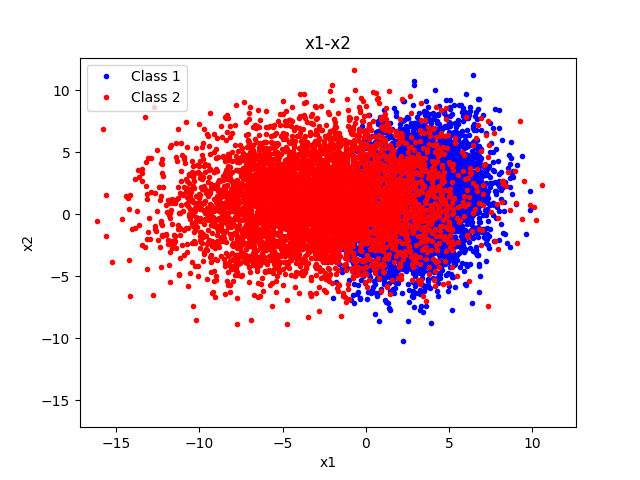
\includegraphics[width=0.45\textwidth]{x1-x2}
	\label{absorbing}
	}
	\subfigure[y1-y2]{
	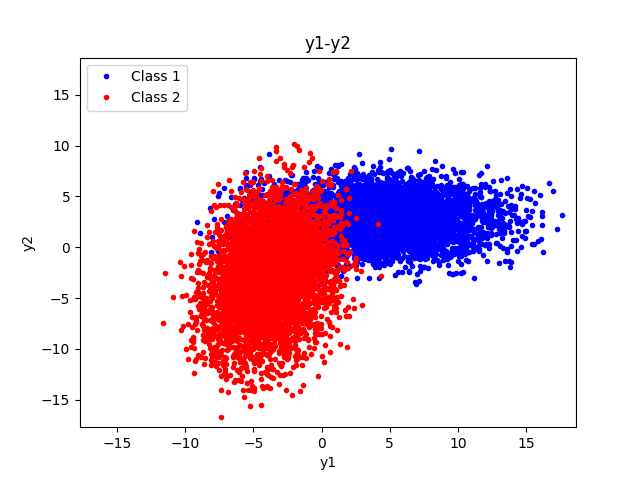
\includegraphics[width=0.45\textwidth]{y1-y2}
	\label{absorbing}
	}\\
	\subfigure[z1-z2]{
	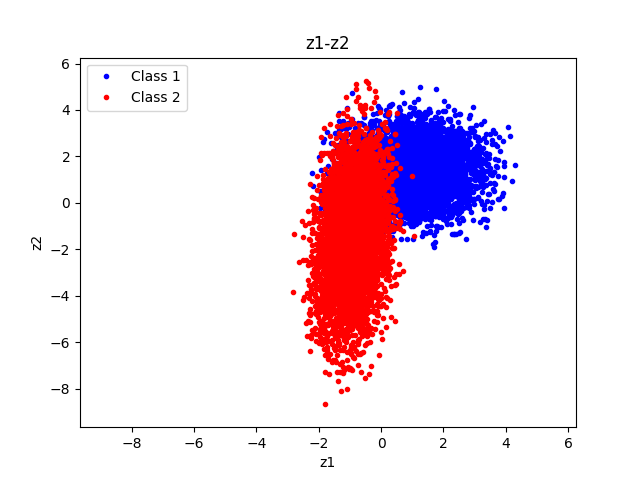
\includegraphics[width=0.45\textwidth]{z1-z2}
	\label{absorbing}
	}
	\subfigure[v1-v2]{
	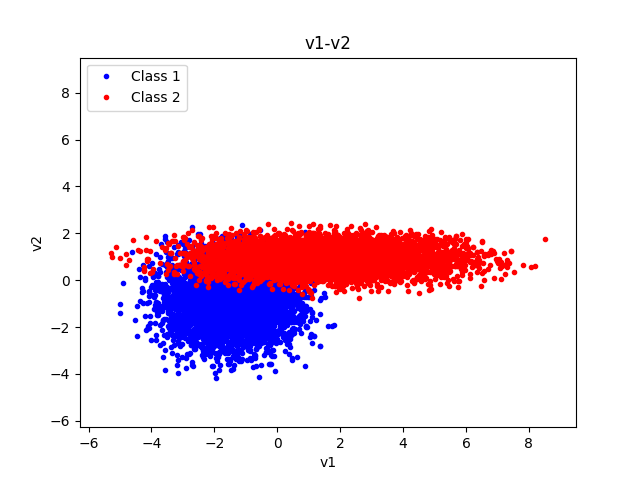
\includegraphics[width=0.45\textwidth]{v1-v2}
	\label{absorbing}
	}
\end{center}
\caption{Transitions of (d1-d2) from X to V}
\end{figure}

\begin{figure}
\begin{center}
	\subfigure[x1-x3]{
	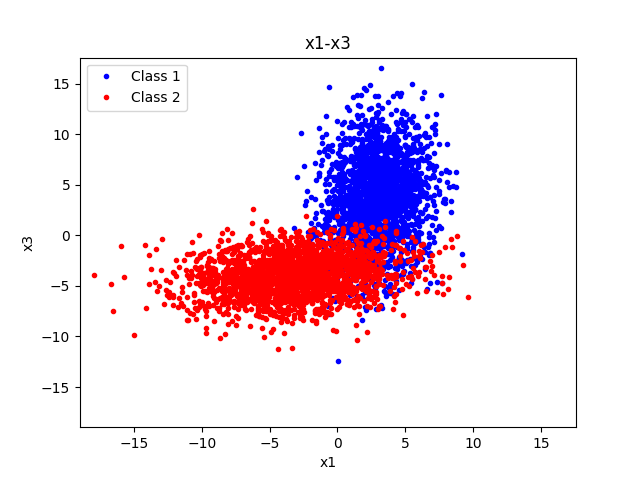
\includegraphics[width=0.45\textwidth]{x1-x3}
	\label{absorbing}
	}
	\subfigure[y1-y3]{
	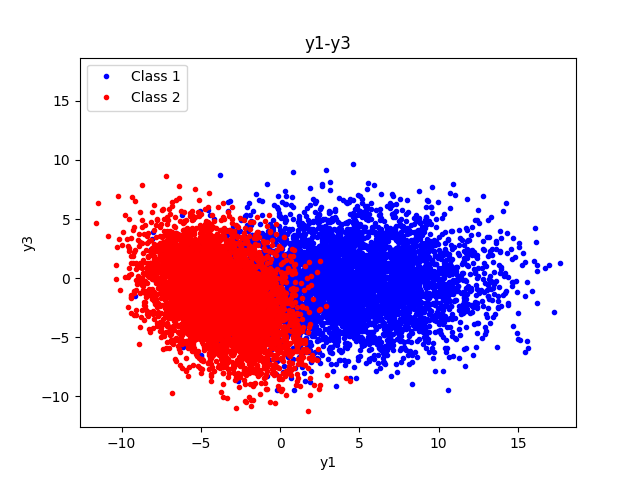
\includegraphics[width=0.45\textwidth]{y1-y3}
	\label{absorbing}
	}\\
	\subfigure[z1-z3]{
	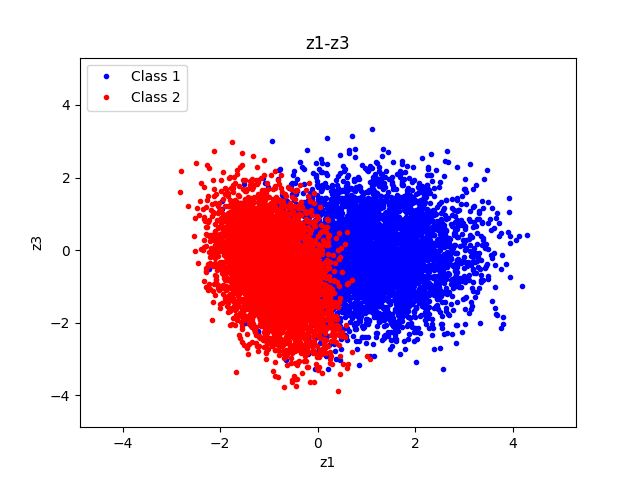
\includegraphics[width=0.45\textwidth]{z1-z3}
	\label{absorbing}
	}
	\subfigure[v1-v3]{
	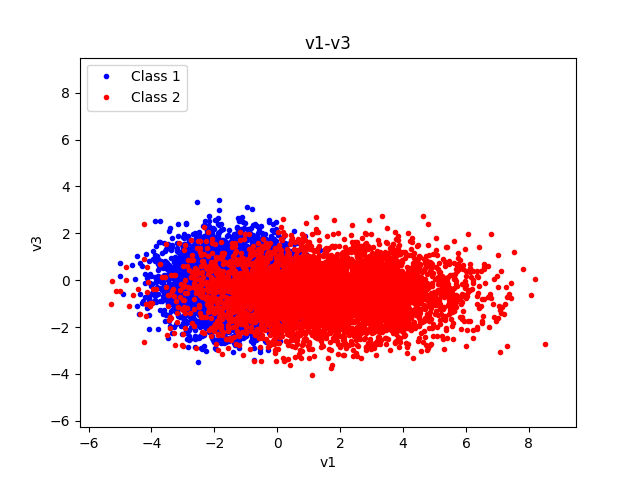
\includegraphics[width=0.45\textwidth]{v1-v3}
	\label{absorbing}
	}
\end{center}
\caption{Transitions of (d1-d3) from X to V}
\end{figure}

\begin{figure}
\begin{center}
	\subfigure[x2-x3]{
	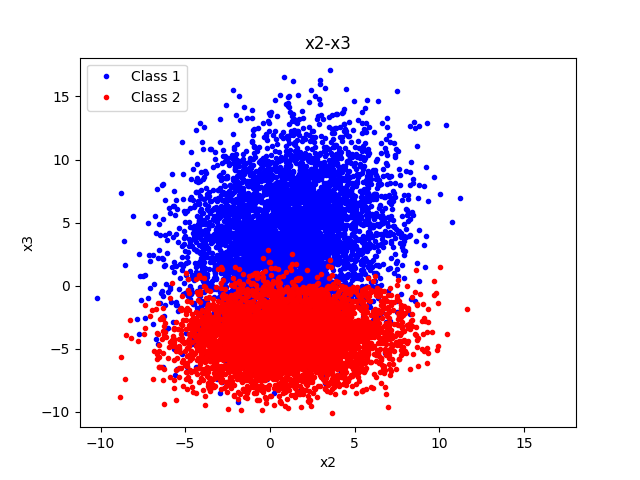
\includegraphics[width=0.45\textwidth]{x2-x3}
	\label{absorbing}
	}
	\subfigure[y2-y3]{
	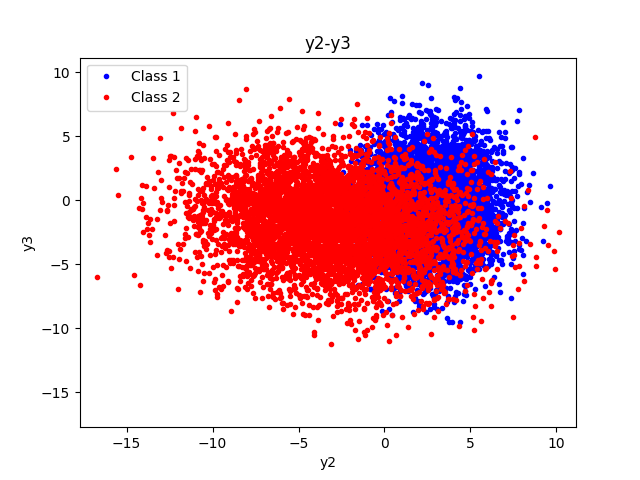
\includegraphics[width=0.45\textwidth]{y2-y3}
	\label{absorbing}
	}\\
	\subfigure[z2-z3]{
	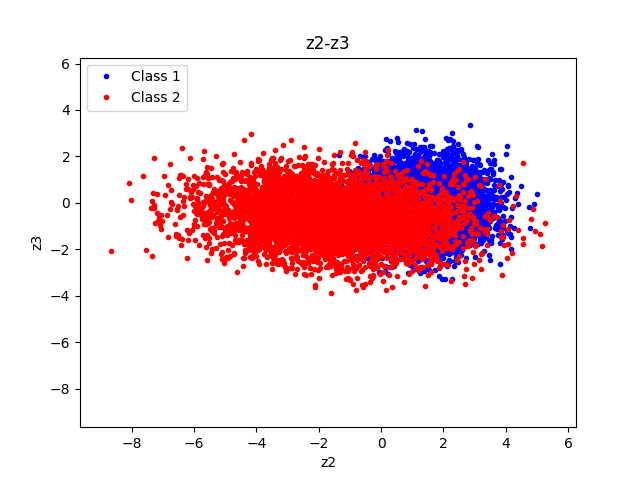
\includegraphics[width=0.45\textwidth]{z2-z3}
	\label{absorbing}
	}
	\subfigure[v2-v3]{
	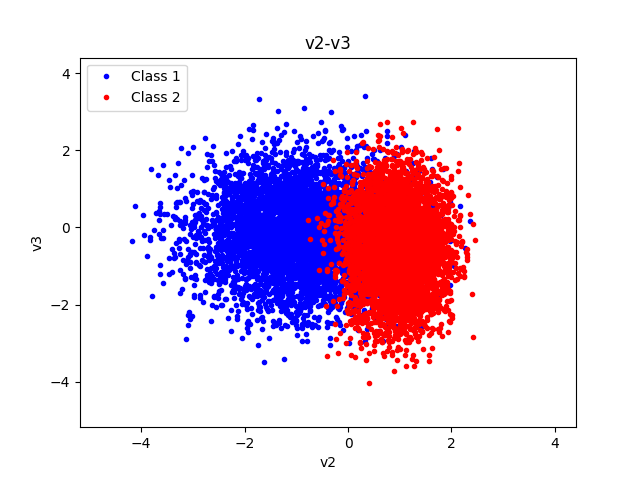
\includegraphics[width=0.45\textwidth]{v2-v3}
	\label{absorbing}
	}
\end{center}
\caption{Transitions of (d2-d3) from X to V}
\end{figure}

\begin{figure}
\begin{center}
	\subfigure[x-3D]{
	\includegraphics[width=0.45\textwidth]{X-3D}
	\label{absorbing}
	}
	\subfigure[y-3D]{
	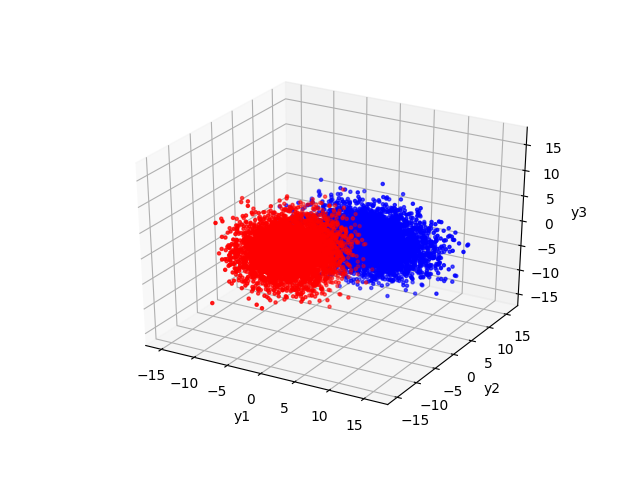
\includegraphics[width=0.45\textwidth]{y-3d}
	\label{absorbing}
	}\\
	\subfigure[z-3D]{
	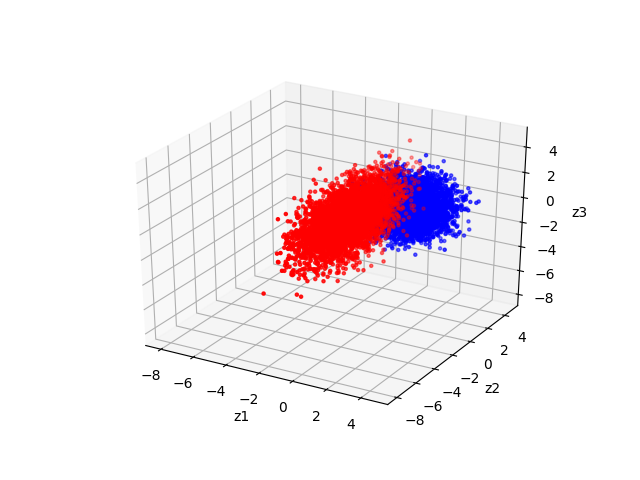
\includegraphics[width=0.45\textwidth]{z-3d}
	\label{absorbing}
	}
	\subfigure[v-3D]{
	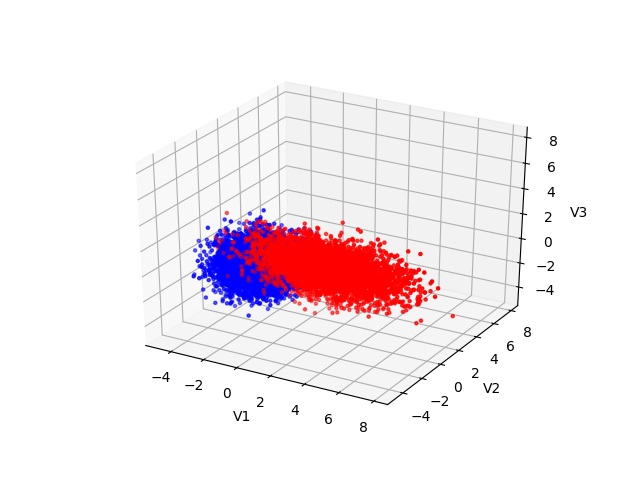
\includegraphics[width=0.45\textwidth]{v-3d}
	\label{absorbing}
	}
\end{center}
\caption{Transitions in 3D from X to V}
\end{figure}


\end{document}  








